\documentclass[12pt]{article}
\usepackage[utf8]{inputenc}
\usepackage{graphicx}
\usepackage{amsmath}
\usepackage{hyperref}
\usepackage{amsfonts}
\usepackage{amssymb}
\usepackage{graphicx}
\usepackage{subcaption}
\usepackage{float}
\usepackage{tikz}
\usepackage{listings}
\usepackage{color}
\usepackage{parskip}
\usepackage{hyperref}
\hypersetup{
    colorlinks=true,
    linkcolor=black,
    citecolor=black,
    filecolor=black,
    urlcolor=black
}
\usepackage[left=1in,right=1in,top=1in,bottom=1in]{geometry}

\title{Rotacrypt: Rotational Mechanics as a Cryptographic Primitive}
\author{Teo Honda Scully}
\date{}

\begin{document}

\maketitle

\begin{abstract}
...TBD...
\end{abstract}

\tableofcontents

\newpage

\section{Introduction}
<...>

\subsection{Review of Rubik's Cubes}
Ah, the Rubik's Cube—the iconic toy that bedevils and delights in equal measure. Born from the ingenious mind of Ernő Rubik in 1974, it's more than just a puzzle. Forget mere child's play; this cube is chaos in the physical. Just kidding. To go from the state of chaos to order, one only needs to know a solving protocol of which many exist.

Max Park, the current world record holder (11 June 2023) for the 2-handed solve, obliterated the cube in a mind-blowing 3.13 seconds. Lucky scramble? Hardly. Yiheng Wang, who holds the world record average-of-five, clocks in at a dizzying 4.48 second mean solve time throughout the five solves.\footnote{An average-of-five is determined by taking the average of the three "middle" solves in a session of five scramble. In other words, the worst and best solve time are dropped from the calculation for the average.} And no, I won't depress you by mentioning his tender age of nine years old. But let's not divert. The Rubik's Cube--a mathematical marvel and a cipher waiting to be cracked. \\

\begin{figure}[h]
    \centering
    \begin{minipage}[c]{0.2\textwidth}
        \includegraphics[scale=0.1]{cube.png}
    \end{minipage}
    \begin{minipage}[c]{0.2\textwidth}
        \includegraphics[scale=0.1]{core_r_highlight.png}
    \end{minipage}
    \begin{minipage}[c]{0.05\textwidth}
        \centering
        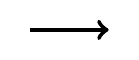
\begin{tikzpicture}
            \draw [->, ultra thick] (0,0.5)--(1,0.5);
        \end{tikzpicture}
    \end{minipage}
    \hspace{0.5cm}
    \begin{minipage}[c]{0.2\textwidth}
        \includegraphics[scale=0.1]{cube_r.png}
    \end{minipage}
    \begin{minipage}[c]{0.2\textwidth}
        \includegraphics[scale=0.1]{core_r_transform.png}
    \end{minipage}
    \caption{A visualization of the \textit{R} operation (rotating the right layer clockwise).}
\end{figure}

Let's dive into the details of the mechanics of the 3x3x3 puzzle. The cube boasts centers, edges, and corners. These center pieces serve as the invariant axis around which the peripheral cubies rotate. The six unit colors are yellow, blue, red, green, orange, and white.

\begin{figure}[h]
    \hfill 
    \begin{minipage}[c]{0.2\textwidth} 
        \centering
        \includegraphics[scale=0.1]{core.png}
    \end{minipage}
    \hfill 
    \begin{minipage}[c]{0.59\textwidth} 
        \vspace*{\fill} 
        A visualization of a 3x3x3 cube. The cube has 6 faces, each with 9 stickers. Notably, this means that there exists 54 different unit tiles on the cube. The cube has 43,252,003,274,489,856,000 possible states.\footnotemark
        \vspace*{\fill}
    \end{minipage}
    \hfill 
\end{figure}
\footnotetext{This number is calculated by considering the \( 8 \) corners, each with \( 3 \) orientations, and the \( 12 \) edges, each with \( 2 \) orientations.}

For instance, if the cube is held with a yellow top and blue front, the red and orange faces will invariably be to the right and left, respectively. In fact, the red and orange center pieces will \textit{always} be opposites, as will the blue-green and white-yellow pairs of center pieces.\\

With fixed center pieces, this means that a static orientation, such as holding the cube with the yellow face on the top layer and the blue face on the front layer (as pictured above) yields an orientation in which the red face will always be to the right, the green face always to the left,

\begin{figure}[H]
    \hspace{20pt}
    \begin{minipage}{.3\textwidth}
        \includegraphics[scale=0.1]{cube.png}
    \end{minipage}%
    \begin{minipage}{.6\textwidth}
        A visualization of a 3x3x3 cube. The cube has 6 faces, each with 9 stickers. Notably, this means that there exists 54 different unit tiles on the cube. The cube has 43,252,003,274,489,856,000 possible states.
    \end{minipage}
    
    \vspace{20pt}
    
    \hspace{20pt}
    \begin{minipage}{.3\textwidth}
        \includegraphics[scale=0.1]{core.png}
    \end{minipage}%
    \begin{minipage}{.6\textwidth}
        The six colors of the cube are Yellow, Blue, Red, Green, Orange, and White. The cube has 6 center pieces, and they are permanently fixed in place. The center pieces are the only pieces that have a single color, and they do not move when the cube is being solved.\\
    \end{minipage}
\end{figure}

The center pieces are permanently affixed to the core. These center pieces serve as the invariant axis around which the peripheral cubies rotate. 



\subsection{Scheme Overview}
<...>

\subsection{Intended Usage}
<...>

\section{3x3x3 Implementation}
<...>

\subsection{Data Structure Breakdown}
<...>

\subsection{Augmented SPEFFZ Mapping}
<...>

\subsection{Cyclic Transformations}

\section{Key Generation}
<...>

\subsection{4-Cube Initialization}
<...>

\subsection{Master-Key Serialization}
<...>

\subsection{Sub-Key Generation}
<...>

\section{Encryption}
<...>

\subsection{Plaintext Setup With S-Box Transformations On Chunks}
<...>

\subsection{Cube Mapping Procedure}
<...>

\subsection{Encryption Algorithm}
<...>

\section{Decryption}
<...>

\end{document}
